\section{Results}

\subsection{Case study}
At this point, it is possible to study a wide variety of flight configuration and situations. To keep the study consice we will limit our analysis to the situation of engine failure at take off with landing gear retracted as described by CS25.121, CS25.147 and CS12.149 \cite{CS25}. The previous rules set the requirements on the climb angle, directional control and $V_{MC}$ in case of one or multiple engine failure at take-off. Although this manner bounds the study to only one flight phase, a good ensight is given on the tool efficiency to compare aircraft configuration and potential of differential thrust.

The certification rules indicate different flight conditions for twin engine and aircraft with more than four engines. The main differences are resumed in table~\ref{tab:DiffTwinMulti}. %CS25.121 states the following flight conditions:
\begin{table}[hbt]
	\caption{\label{tab:DiffTwinMulti} Certification differences between twin-engines and more than four engines, \cite{CS25}} 
	\centering
	\begin{tabular}{l|l|c}
		Parameters & Twin engine & More than four engines\\
		\hline
		Gradient of climb, critical engine inoperative & $\leq 2.4\%$ & $\leq 3.0\%$\\
		Heading change of $15\degree$ at 1.3$V_{SR_1}$& One engine inoperational & Two critical engines inoperational\\
		$V_{MC} < 1.13 V_{SR}$ & One engine inoperative & One critical engine inoperative \\
	\end{tabular}
\end{table}

It is of interest to investigate the most defavorable situation for differential thrust which is clearly at a $3\%$ climb angle. The same climb angle is imposed for all configuration even if it disadvantage the original ATR, it allows to compare aircraft at an identical flight situation.

A total of four configurations are studied to capture the overall changes that differential thrust and VT reduction bring to the aircraft. These configurations are resumed in table~\ref{tab:ConfigurationStudied}. It must be stressed that velocities are calculated from publicly available data and thus are only indicative.

\begin{table}[hbt]
	\caption{\label{tab:ConfigurationStudied} Aircraft Configurations}
	\centering
	\begin{tabular}{l|c|c|m{3cm}|m{3cm}}
		Parameters & Original ATR72 & DEP ATR72 & DEP ATR72 Differential Thrust & DEP ATR72 Differential Thrust and small VT\\
		\hline
		Engines & 2 & 12 & 12 & 12\\
		Inoperative engines & 1 & 3 & 3 & 3\\
		VT area & $S_{v_0}$ & $S_{v_0}$ & $S_{v_0}$ & $0.7 S_{v_0}$\\
		Rudder allowed & Yes & Yes & No & No\\
		Gradient of climb & $3.0\%$ &$3.0\%$ & $3.0\%$ & $3.0\%$\\
		Turn rate, $\Omega$ (rad/s)& 0 & 0& 0&0\\
		
		\hline
		\multicolumn{5}{c}{Additional parameters} \\
		\hline
		$V_{\textrm{app}}$=$1.13V_{\textrm{app}}$ (m/s)& \multicolumn{4}{c}{56}\\
		$V_{\textrm{sr}}$ (m/s)& \multicolumn{4}{c}{50.5}\\
		$1.3V_{\textrm{sr}}$ (m/s)& \multicolumn{4}{c}{65}\\
		VT stall limit & \multicolumn{4}{c}{$\beta=15\degree$}\\
		\hline
		\multicolumn{5}{c}{Flight parameters for throttle repartition and rudder deflection}\\
		\hline
		$\beta$ & \multicolumn{4}{c}{$0\degree$}\\
		V(m/s) & \multicolumn{4}{c}{60}\\
	\end{tabular}
\end{table}


For each configuration an equilibrium map is built by swapping side slip angle and flight velocity. Along the rudder deflection and throttle repartition of a single equilibrium point is presented. Side slip angle and velocity for this point is shown in table~\ref{tab:ConfigurationStudied}

%\begin{itemize}
%\item Climb gradient with one engine inoperative may not be less than 2.4\% for twin engines
%\item Climb gradient with one engine inoperative may not be less than 3\% for aircrafts with four engines or more.
%\end{itemize}

\subsection{Flight envelop map}
The flight envelops along with the accompaning throttle repartition and rudder deflection are shown in Fig~\ref{MapOrignialTwin+DEP} to Fig~\ref{fig:DEPfin07_15enginesMap+Defl}.

First the baseline ATR72 is presented in Fig~\ref{fig:originalfin1_3engine} and the trim inputs in Fig~\ref{fig:Defloriginalfin1_3engine}. The climb gradient is slightly unfavorable for this configuration nevertheless, one can clearly see the compliance with the controlability at low velocity and the $15\degree$ margin at $1.3V_{SR}$

\begin{figure}[hbt!]
	\centering
	\begin{subfigure}{0.49\textwidth}
		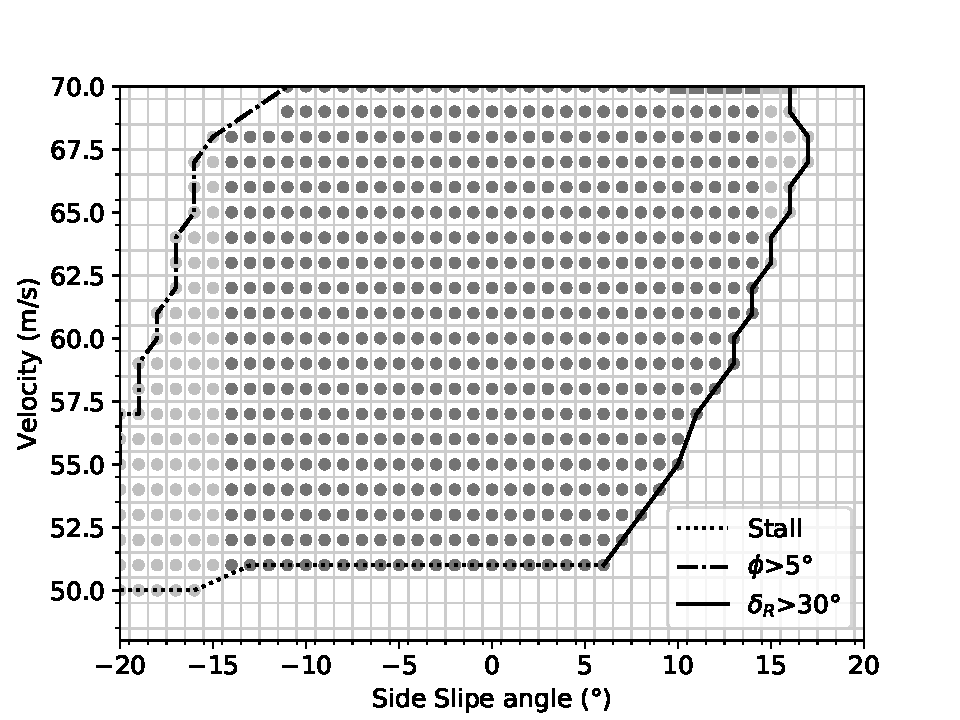
\includegraphics[width=0.95\textwidth]{originalMapBetaVelfin1Eng3RudFalse}
		\caption{Original ATR72 with one engine failure.}
		\label{fig:originalfin1_3engine}
	\end{subfigure}
	\begin{subfigure}{0.49\textwidth}
		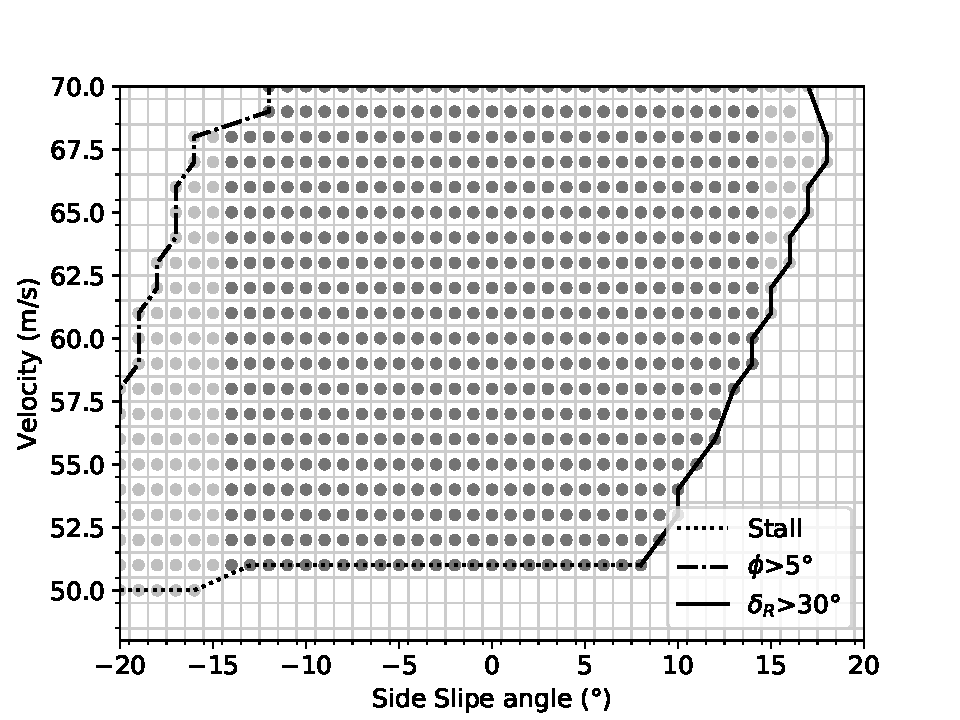
\includegraphics[width=0.95\textwidth]{originalMapBetaVelfin1Eng15RudFalse}
		\caption{ATR with 12 engines, three inoperatives.}
		\label{fig:originalfin1_15engine}
	\end{subfigure}
	\caption{Original ATR with \ref{fig:originalfin1_3engine} twin engine, one inoperational and \ref{fig:originalfin1_15engine} twelve engines, three inoperational. Only the rudder is used to compensate the yawing moment.} \label{MapOrignialTwin+DEP}
\end{figure}

\begin{figure}
	\begin{subfigure}{0.49\textwidth}
		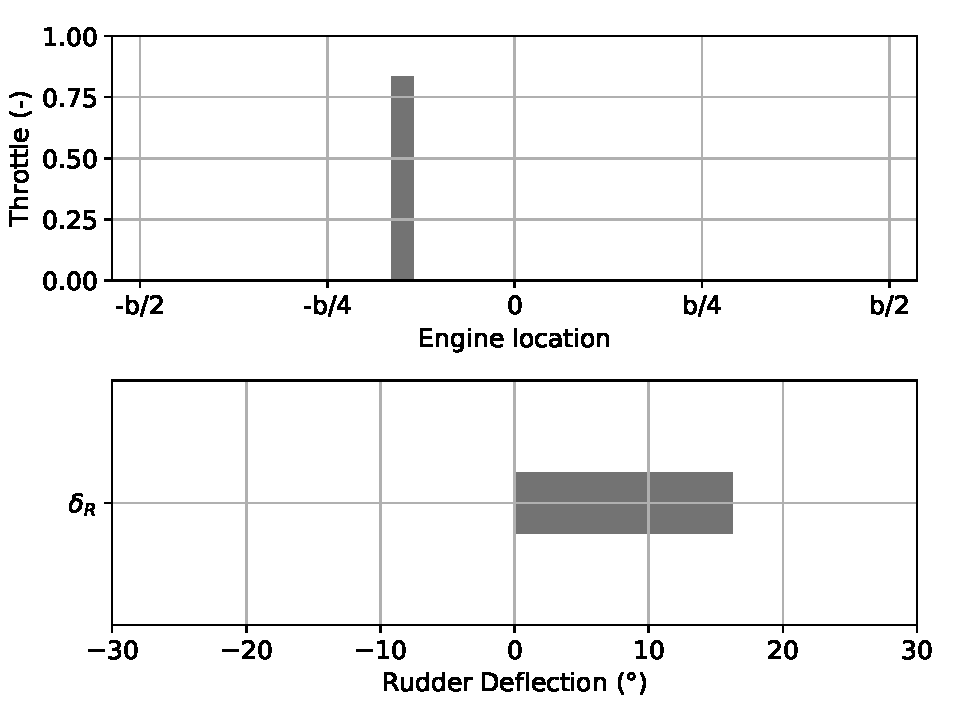
\includegraphics[width=0.95\textwidth]{Defloriginalfin1Eng3RudFalse}
		\caption{Original ATR72 with one engine failure.}
		\label{fig:Defloriginalfin1_3engine}
	\end{subfigure}
	\begin{subfigure}{0.49\textwidth}
		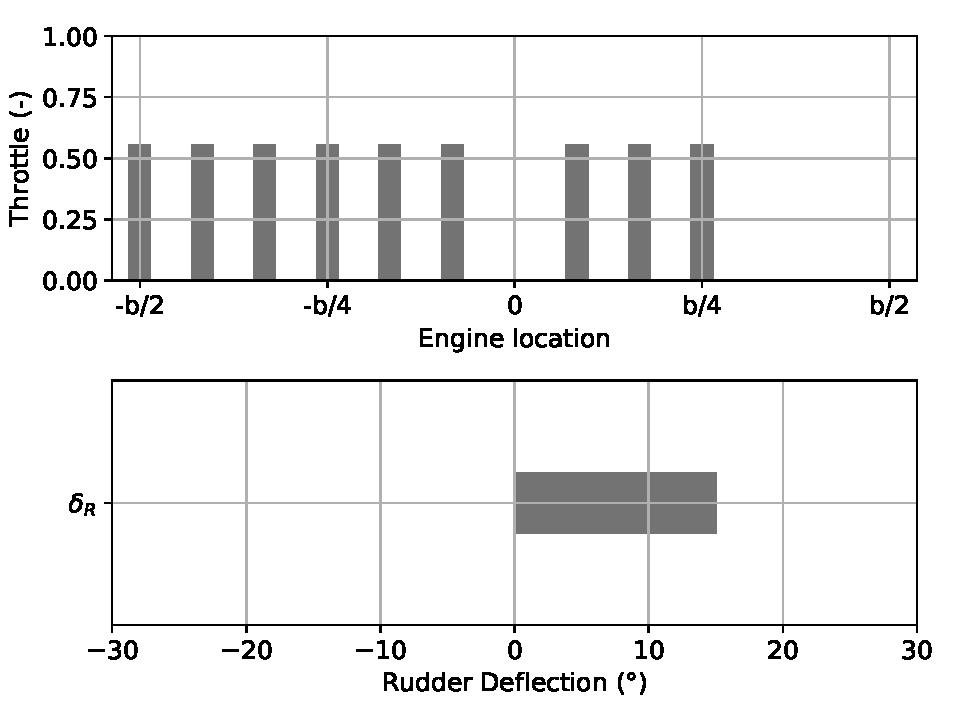
\includegraphics[width=0.95\textwidth]{Defloriginalfin1Eng15RudFalse}
		\caption{Original ATR with twelve engines, three inoperatives.}
		\label{fig:Defloriginalfin1_15engine}
	\end{subfigure}
	\caption{Throttle level and rudder deflection for trim at V=60m/s, $\beta=0$} \label{DeflOrignialeNoDiffThrust}
\end{figure}

\begin{figure}[hbt!]
		\centering
		\begin{subfigure}{0.49\textwidth}
			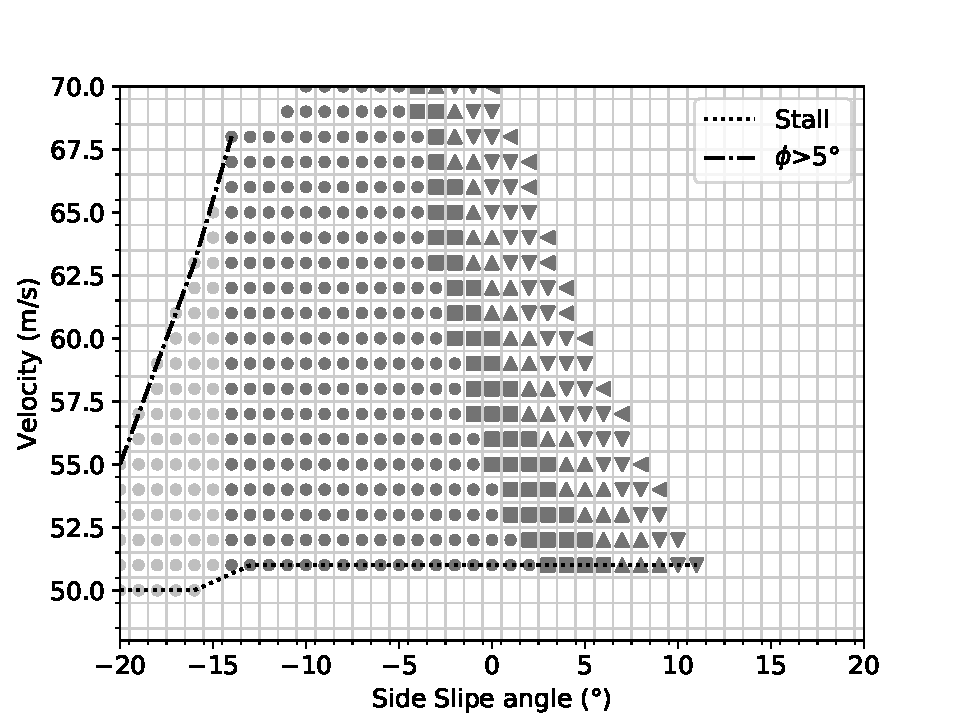
\includegraphics[width=0.95\textwidth]{DEPoriginalMapBetaVelfin1Eng15RudTrue}
			\caption{Flight envelop, ATR with 12 engines, three inoperatives.}
			\label{fig:DEPoriginalfin1_15engine}
		\end{subfigure}
		\begin{subfigure}{0.49\textwidth}
			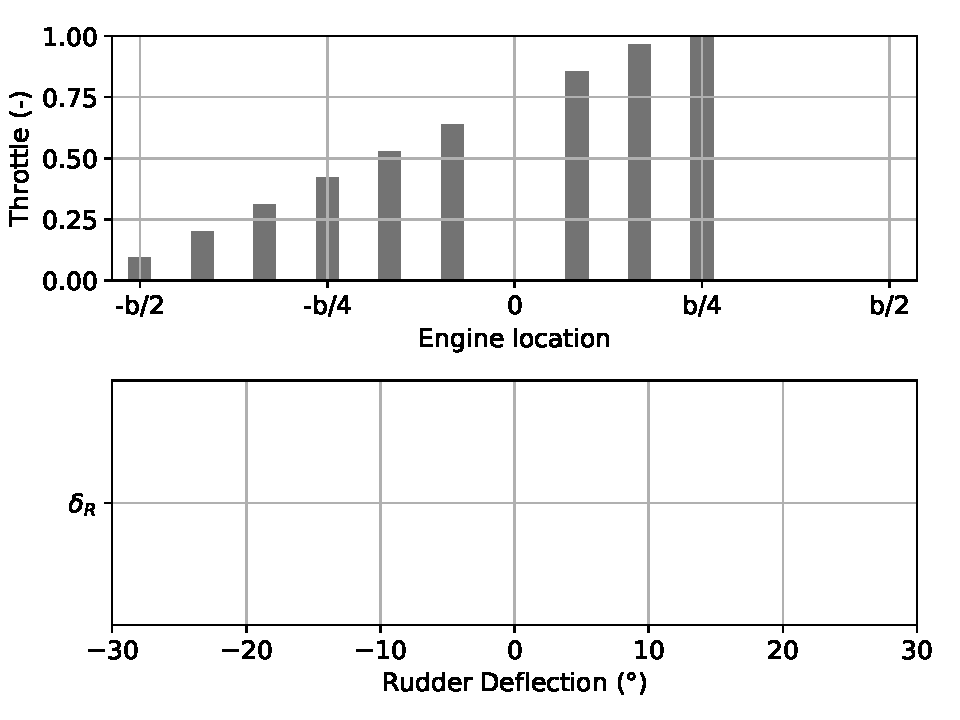
\includegraphics[width=0.95\textwidth]{DeflDEPoriginalfin1Eng15RudTrue}
			\caption{Throttle level and Rudder deflection at 60m/s and $\beta=0\degree$, ATR72 with 12 engines, three inoperatives.}
			\label{fig:DeflDEPoriginalfin1_15Eng}
		\end{subfigure}
		\caption{ATR72 using only differential thrust. Circles indicate an equilibrium point, rectangle indicate an equilibrium with at least one engine at saturation (full throttle)}\label{DEPfin1_15engMap+Defl}
\end{figure}

\begin{figure}[hbt!]
	\centering
	\begin{subfigure}{0.49\textwidth}
		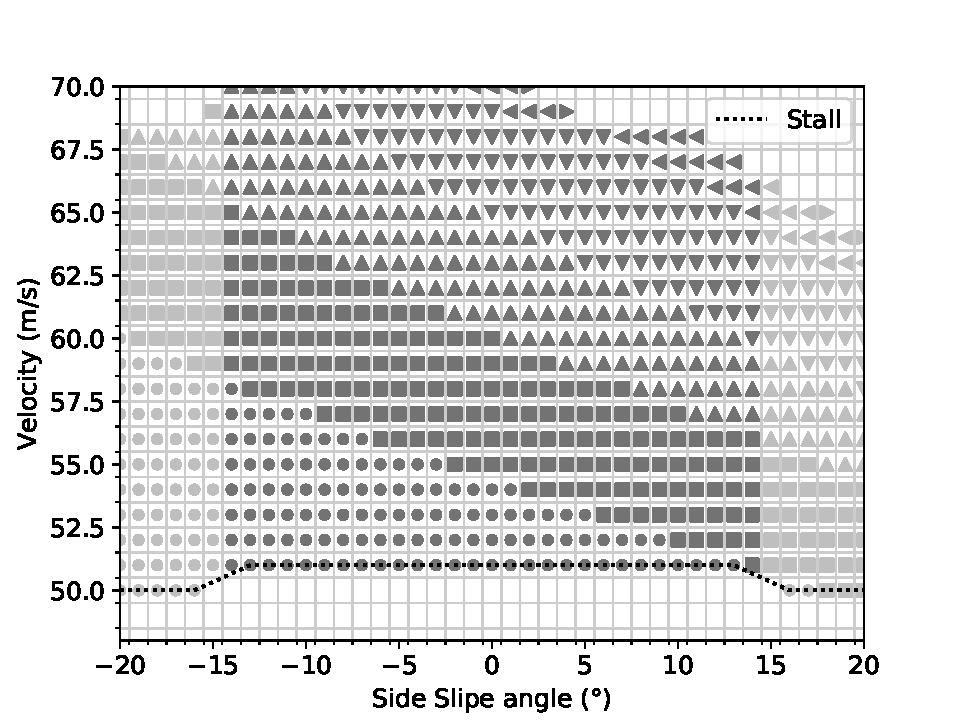
\includegraphics[width=0.95\textwidth]{DEPoriginalMapBetaVelfin07Eng15RudTrue}
		\caption{Circles indicate an equilibrium point, rectangle indicate an equilibrium one engine at saturation (full throttle), up triangles two engines, down triangle three engines etc...}
		\label{fig:DEPoriginalfin07_15engine}
	\end{subfigure}
	\begin{subfigure}{0.49\textwidth}
		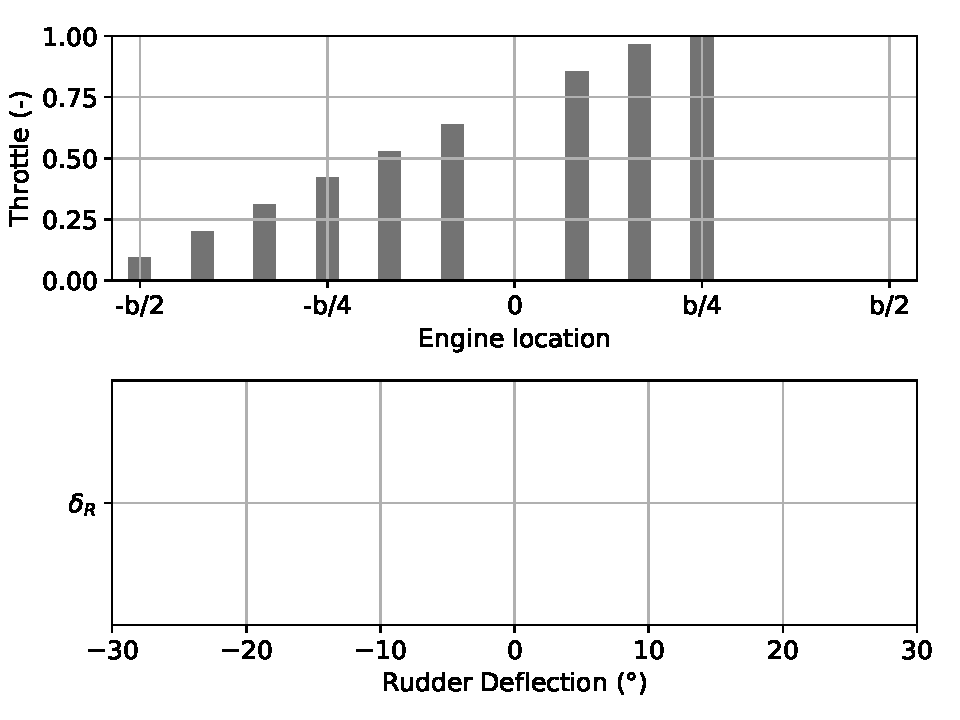
\includegraphics[width=0.95\textwidth]{DeflDEPoriginalfin07Eng15RudTrue}
		\caption{Throttle level and Rudder deflection at 60m/s and $\beta=0\degree$, ATR72 with 12 engines, three inoperatives, $S_v=0.7S_{v_0}$.}
		\label{fig:DeflDEPoriginalfin07_15Eng}
	\end{subfigure}
	\caption{ATR with 12 engines, three inoperatives and $S_v=0.7S_{v_0}$. Rudder not used.}\label{fig:DEPfin07_15enginesMap+Defl}
\end{figure}

%----- Study Case -----
%One original ATR72 at take off without failed engine next to the same ATR72 at Take off with SEF:
%	Shows that Vmc is found for take off,
%	Show that control is maintained at 1.3Vsr (=15° yaw toward inoperative engine)
%	shows that no equilibrium exists,
%	eventually show the degradation of equilibrium with reduced VT
%	Show the engine saturation at high speed

%Show the same ATR with distributed propulsion:
%	Show input histogramme with and without rudder
%	Show map without rudder and with small rudder
%	Show map with small fin and rudder
%
%At take off means :
%	3% slope for more than 4 engine condition, 
%	2.4 % for twin engine with landing gear retracted (CS.25.121)
%	Not necessarly full power but explore by going higher (in speed mostly)
%	0 altitude
%Maybe replace velocity scale by Vsr, 1.3Vsr etc... as defined by CS

% ATR at 21.5T Vapp=56m/s if it is 1.13Vsr then Vsr=49.55m/s, 1.3Vsr=64.4m/s
% Eventually look at the 20° turns requirement from the certif

%
%Determine 1.3V_{sr} for CS25.147 stating 15° yaw in the direction of the inoperative engine.
%STATE MINIMUM DRAG and 